\chapter{Synapsis}

\section{Setup e Avvio}

Passi da seguire per configurare l'ambiente idoneo a Synapsis:
\begin{enumerate}
    \item Installare \href{https://www.scala-sbt.org/}{sbt};
    \item Scaricare il repository \textbf{mas-ge-middleware} utilizzando i link nella sezione \ref{materiale_online};
    \item Da terminale, navigare fino alla cartella \textbf{synapsis-middleware} interna al repository;
    \item Utilizzare il comando \textbf{sbt compile} per effettuare una prima compilazione del progetto.
\end{enumerate}

Passi da seguire per avviare Synapsis:
\begin{enumerate}
    \item Da terminale, navigare fino alla cartella \textbf{synapsis-middleware} interna al repository;
    \item Utilizzare il comando \textbf{sbt run} per avviare il progetto.
    \item Aprire un browser ed andare all'indirizzo \href{http://localhost:9000/}{http://localhost:9000/} per verificare l'effettivo avvio del progetto\footnote{La pagina principale è ancora un template senza funzionalità, serve solo a capire se il middleware è online}.
\end{enumerate}

\section{MockActor} \label{mock_actor}
Il MockActor è stato realizzato con l'obiettivo di velocizzare la fase di sviluppo, dato che permette di creare "finti" (dall'inglese "mock") attori che sostituiscono gli attori realmente collegati ad un'entità esterna. 

\medskip

Lo scenario ideale per l'utilizzo di questa modalità è quello di sviluppatori in grado di utilizzare solo una tecnologia, tra Unity e JaCaMo, e che attraverso la realizzazione di MockActor specifici riescano a sopperire alla necessità di uno sviluppo simultaneo.

\subsection{Come utilizzare il MockActor}

I passi da seguire per realizzare "finti" attori sono i seguenti:

\begin{enumerate}
    \item Creare una classe java che estenda MockActor,
    \item Posizionare la classe dentro il package \textbf{actor.mock} presente nel middleware,
    \item Implementare i metodi astratti come mostrato nel listato \ref{codiceMock}.
\end{enumerate}

\lstinputlisting[label={codiceMock},caption={Esempio di attore che estende la classe \textit{MockActor}},language=Java]{code/TestMock.java}

Il metodo \textit{parseIncomingMessage}, invocato ad ogni messaggio ricevuto dall'attore, permette allo sviluppatore di decidere come gestire tali messaggi che possono essere azioni o percezioni inviate dall'attore controparte e, quindi dall'entità esterna collegata al middleware.

\medskip

A disposizione dello sviluppatore sono presenti alcuni metodi, già implementati all'interno della classe \textit{MockActor}, per interagire con l'attore controparte (mente/corpo) e quindi con l'entità ad esso collegata. Il listato \ref{metodiMock} contiene tutti i metodi utilizzabili con i relativi commenti. 

\lstinputlisting[label={metodiMock},caption=Metodi per interagire con la controparte,language=Java]{code/MockActorAPI.java}

Il metodo \textit{sendResponse} è la condizione per inviare una generica risposta alla controparte e, quindi, utilizzabile per inviare un messaggio al corpo o alla mente. \'E da notare la presenza di interazioni predefinite dal punto di vista del contenuto del messaggio, difatti tutti i metodi che finiscono per \textit{Action} e per \textit{Perception} inseriscono automaticamente il contenuto principale del messaggio (sezione \ref{protocollo_messaggi}). Ad esempio, nel caso di \textit{searchAction} il contenuto sarà \textit{"search"}. L'obiettivo di questi metodi è quello di mettere subito a disposizione dello sviluppatore un primo set di Azioni e Percezioni già associate a una logica predefinita nelle restante parte del sistema.

\subsection{Architettura del sistema con MockActor}

Questa modalità di fast prototyping, modifica la architettura del sistema (Figure \ref{mock_actor_body} e \ref{mock_actor_mind}) in basa a quale tipologia di \textit{MockActor} viene utilizzato.

\begin{figure}[H]
\centering
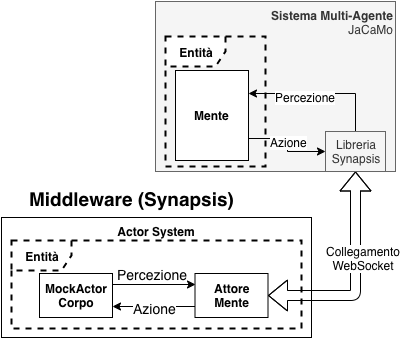
\includegraphics[width=0.6\textwidth]{figures/architettura_mock_actor_body.png}
\caption{Architettura con un MockActor di tipo \textit{body}}
\label{mock_actor_body}
\end{figure}

Con l'utilizzo di un "finto" attore che rappresenta la parte di entità "corpo" l'architettura del sistema si modifica di conseguenza, visto che viene meno la parte di Game Engine (GE). Le percezioni e le risposte alle azioni ricevute vengono simulate dal \textit{MockActor} di tipo "corpo" realizzato, che potrà essere successivamente sostituito dall'entità "corpo" in futuro realizzata sulla GE.

\begin{figure}[H]
\centering
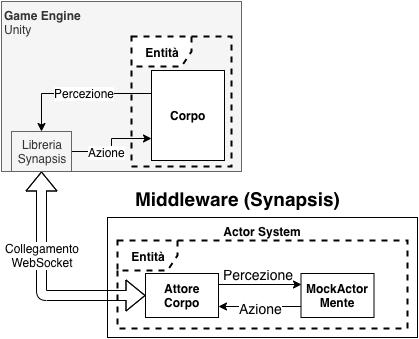
\includegraphics[width=0.6\textwidth]{figures/architettura_mock_actor_mind.png}
\caption{Architettura con un MockActor di tipo \textit{mind}}
\label{mock_actor_mind}
\end{figure}

Con l'utilizzo di un "finto" attore che rappresenta la parte di entità "mente", l'architettura del sistema si modifica di conseguenza, visto che viene meno la parte di Sistema Multi-Agente (MAS). L'autonomia viene simulata dal \textit{MockActor} di tipo "mente" realizzato che potrà essere successivamente sostituito dall'entità "mente" realizzata sul MAS.

\subsection{Istanziare MockActor}

\subsubsection{Istanziare dall'interno del middleware}

Lo sviluppatore ha a disposizione due metodi all'interno della classe \textbf{Application}, che permettono di istanziare uno o più "finti" attori precedentemente realizzati.

\lstinputlisting[label={mockactorapplication},caption={Metodi per istanziare un MockActor nel middleware},language=Java]{code/Application_mock.java}

I metodi \textit{spawnMockActor} e \textit{spawnMockActors} permettono di creare, all'interno del sistema, generici attori dato che accettano classi Java che estendano la classe \textit{MockActor}. Questi metodi, come da listato \ref{mockactorapplication}, vanno utilizzati nel costruttore della classe \textbf{Application} per essere certi di istanziare gli attori all'avvio dell'applicazione.

\subsubsection{Istanziare dall'esterno del middleware}

Per istanziare MockActor runtime sono state fornite delle API nelle rispettive librerie di JaCaMo e Unity che comunicano direttamente con il middleware e permettono la creazione di questi attori attraverso l'invio di un messaggio predefinito.

\medskip

Su Unity è stato realizzato un processo che utilizza l'interfaccia grafica dell'IDE (figura \ref{gui_script}). Collegando al GameObject uno script che estende \textit{SynapsisBody} si ottiene il seguente risultato:

\begin{figure}[H]
\centering
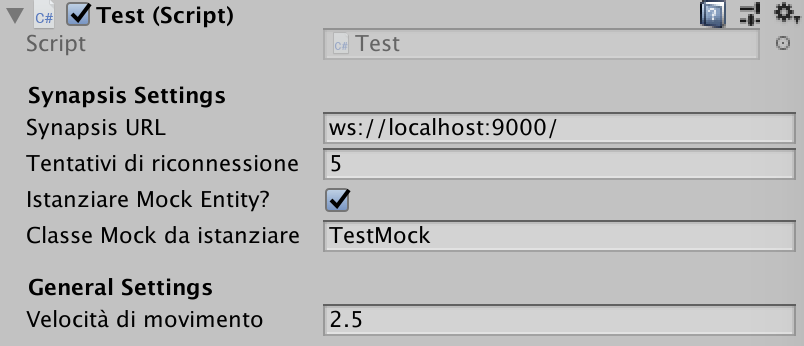
\includegraphics[width=0.7\textwidth]{figures/Unity_Test_editor.png}
\caption{Interfaccia grafica di gestione dello script}
\label{gui_script}
\end{figure}

I parametri \textit{"Istanziare Mock Entity?"} e \textit{"Classe Mock da istanziare"}, permettono al GameObject di creare il messaggio da inviare al middleware appena stabilito il collegamento WebSocket.

\medskip

Per JaCaMo sono presenti due modalità. La prima è effettuabile attraverso l'invocazione di uno specifico metodo presente nell'artefatto \textit{SynapsisMind}.

\lstinputlisting[caption={Metodo per istanziare MockActor dall'artefatto},language=Java]{code/SynapsisMind_istanziare_mock_actor.java}

La seconda utilizza uno specifico plan presente nell'agente \textit{SynapsisBaseAgent} che a loro volta utilizza l'operazione (metodo) del listato precedente.

\lstinputlisting[caption={Piano per istanziare MockActor},language=asl]{code/plan_mock_actor.asl}

In entrambe le situazioni, lo sviluppatore deve fare attenzione a scrivere correttamente il nome della classe da istanziare ed a posizionare la classe Java nel corretto package (actors.mock).


